\label{ch:appendix_jena}

\section{Appendix}

\subsection{Jena}

\begin{table}[!htbp]
\centering
  \caption{Per-flower visitation rates (mean $\pm$ SD) for all focal flower species per 15 minute observation. \textit{Geranium pratense} and \textit{Onobrychis viciifolia} are significantly different from the other three species (pairwise t-test, \textit{p} $<$ 0.001) . Within the two groups, there is no significant difference between the species. }
    \begin{tabular}{l l l l l}
    \toprule
    \textbf {Short} & \textbf{Species} & \textbf{Family} &\textbf{Visitation Rate (Mean)} & \textbf{ $\pm$ SD} \\
    \midrule
    Ger  & \textit{Geranium pratense} & Geraniaceae & 3.05 & 1.5 \\ %109
    Lat  & \textit{Lathyrus pratensis} & Fabaceae & 0.57 & 0.53 \\ %83
    Lot  & \textit{Lotus corniculatus} & Fabaceae & 0.30 & 0.36 \\  % 77
    Ono  & \textit{Onobrychis viciifolia} & Fabaceae & 3.60  &  2.5 \\ % 37
    TP   & \textit{Trifolium pratense} & Fabaceae & 0.16 & 0.23 \\ % 79
    \bottomrule
    \end{tabular}%
\label{tab:VR_spec}
\end{table}%

%%%%%%%%%%%%%%%%%%%%%%%%%%

\begin{table} [!htbp] %results lme
	\centering
	\caption{Results of the linear mixed effect model with per-flower visitation rate as explanatory variable. Floral cover and species richness were not relevant predictors for the model and therefore removed in the model selection process (denDF = 191, R$^{2}$ = 0.53, n = 385)}
	\begin{tabular} { l l c c c}
		\toprule
		\textbf{Response Variable} & \textbf{Explanatory Variables} & \textbf{Df} & \textbf{F-value} & \textbf{\textit{P}} \\
		\midrule
		Per-flower visitation rate   & Species & $4$ & $130.9$ & $<0.0001$\\
		& Frequency 			&  $1$ & $49.3$ & $<0.0001$ \\
		& Frequency$^{2}$ 		&  $1$ & $13.2$ & $0.0026$ \\
		& Frequency$^{3}$ 		&  $1$ & $ 5.8$ &  $0.8145$ \\
		& Frequency x Species &  $4$ & $ 5.2$ &  $0.0005$ \\
		& Frequency$^{2}$ x Species & $4$ & $3.4$ & $0.0097$\\
		& Frequency$^{3}$ x Species & $4$ & $3.4$ & $0.0101$\\
		\bottomrule
	\end{tabular}
	\label{tab:anova}
\end{table}


%%%%%%%%%%%%%%%%%%%%%%%%%%

\begin{figure}  [H] %results lme
\centering
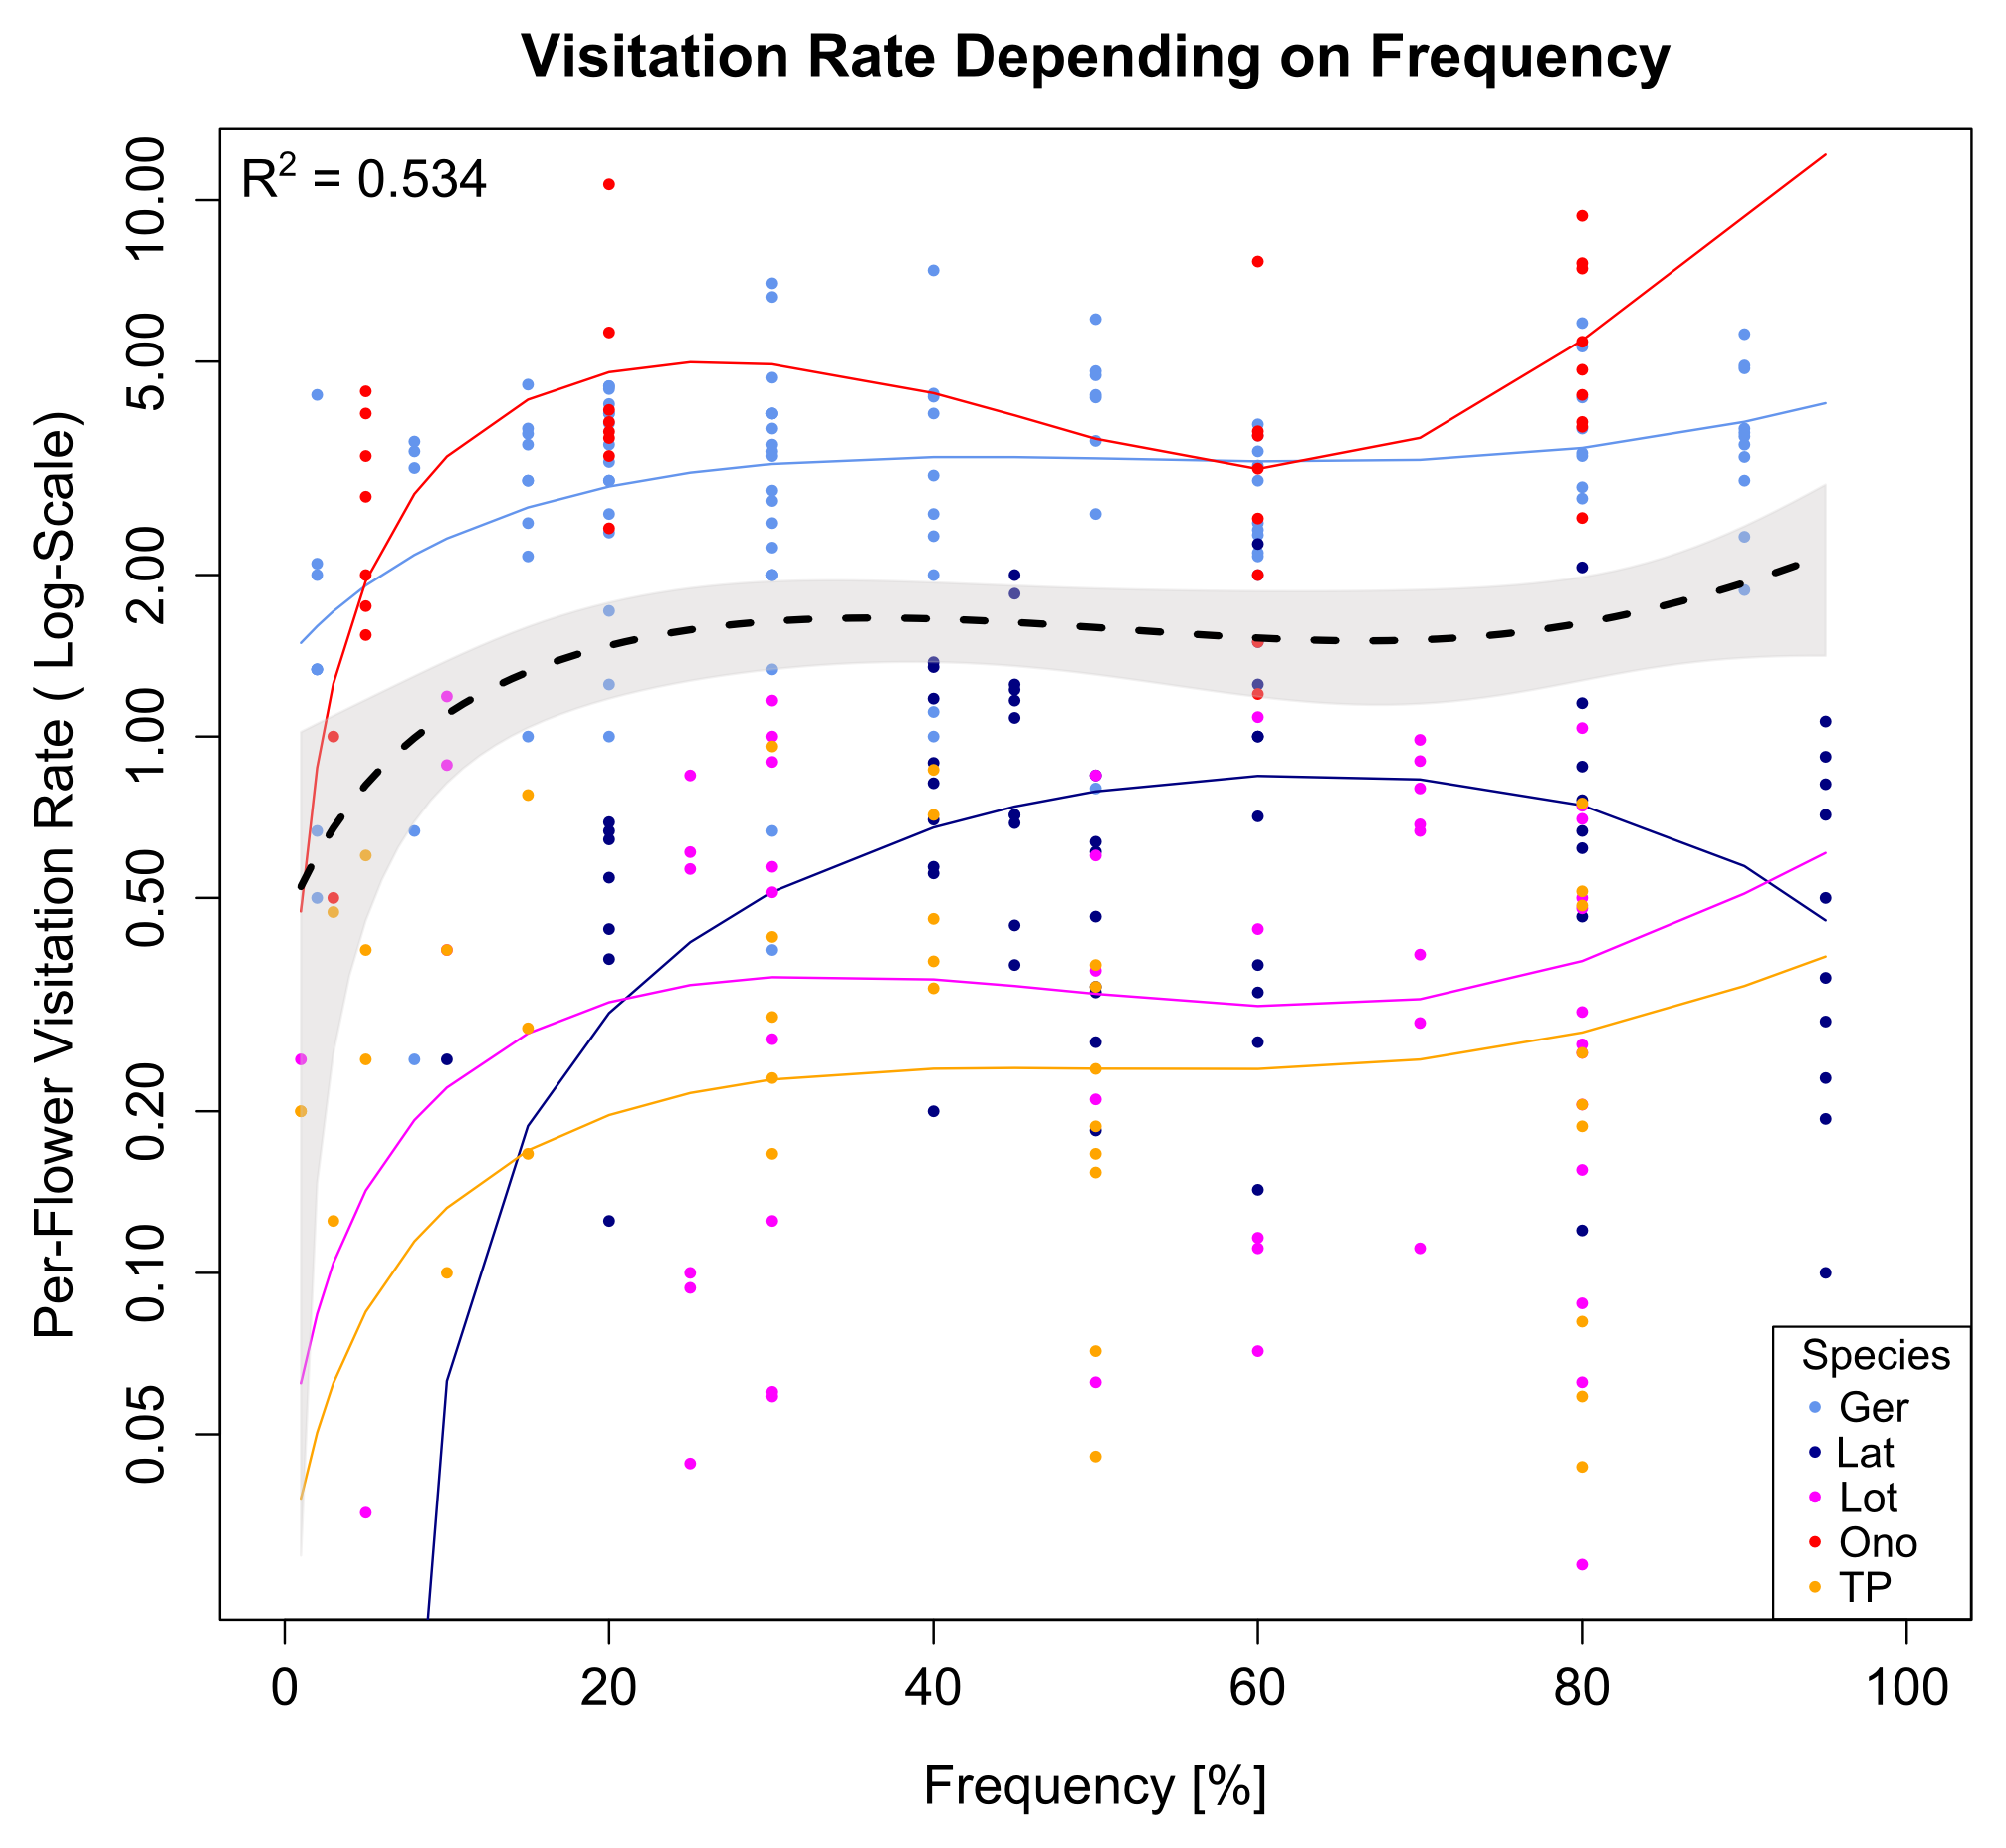
\includegraphics[width=14cm]{Images/LME}
 \caption{Per-flower visitation rates of the five focal species over different frequencies. Each point represents one observation of 15 minutes. The y-axis is plotted on a log scale due to the divergence in attractiveness of the focal species. The linear mixed effect model with Subplot nested in Plot as random factor show a sigmoidal frequency dependence for all species but \textit{Lathyrus pratensis}. Floral cover and species richness were dropped as explanatory variables in the model selection process. R$^{2}$ was calculated with the "r.squaredGLMM"-function of the MuMIn-Package \citep{MuMIn}}
 \label{fig:LME}
\end{figure}

%%%%%%%%%%%%%%%%%%%%%%%%%%
